
 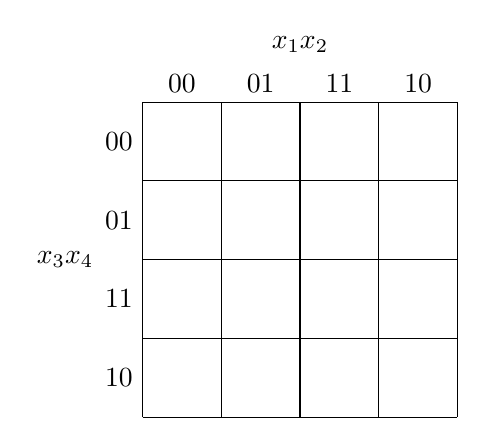
\begin{tikzpicture}[
 pi/.style={fill,draw,circle,minimum size=.1cm},
 pi1/.style={pi,red},
 ]
 \draw (0,0) grid (4,4);
\draw (2,4) node[above=.5cm] {$x_1x_2$}
 	(0,2) node[left=.5cm]  {$x_3x_4$};
\foreach \p/\code in {0/$00$,1/$01$,2/$11$,3/$10$} {
 		\draw[xshift=.5cm] (\p,4) node[above] {\code};
 		\draw[yshift=3.5cm,yscale=-1] (0,\p) node[left]  {\code};
 	}

 		\draw[shift={(.5,.5)},inner sep=.1mm]
 		(3,0) node[]   {$$}
 		(2,0) node[]   {$$}
 		(1,0) node[]   {$$}
 		(3,1) node[]   {$$}
 		(2,1) node[]   {$$}
 		(1,1) node[]   {$$}
 		(0,1) node[]   {$$}
 		(3,2) node[]   {$$}
 		(2,2) node[]   {$$}
 		(1,2) node[]   {$$}
 		(0,2) node[]   {$$}
 		(3,3) node[]   {$$}
 		(2,3) node[]   {$$}
 		(1,3) node[]   {$$}
 		(0,3) node[]   {$$}
 		(0,0) node[]   {$$}
 		
 	
 		;
 		%Beschriftung
 		%	\foreach \p/\code in {2/$11$,3/$10$} {
 		%		\draw[xshift=.5cm] (\p,4) node[above] {\code};
 		%		\draw[yshift=3.5cm,yscale=-1] (0,\p) node[left]  {\code};
 		%	}
 	
 	\end{tikzpicture}
